% TODO: Include the derivation of the damping term and the derivation of \Delta
% \omega instead of using only \omega
\chapter{Synchronous Generators} \label{chap:sg_modeling}

Synchronous generators form the backbone of contemporary power generation,
converting the mechanical energy sourced from fossil fuel combustion or natural
resources like water streams into electrical energy. Their operation at a
constant speed synchronized with the AC power frequency has made them a staple
in the field since the late 19th century.

This chapter delves into the enduring role of synchronous generators, focusing
on their operational intricacies and control strategies. Over the years, various
control methods, including Automatic Voltage Regulation (AVR), Power System
Stabilization (PSS), and Automatic Generation Control (AGC), have been developed
to ensure the stable performance of these machines.

The objective of this chapter is to elucidate key concepts and models associated
with synchronous generators, providing a foundation for understanding their
behavior. For a more detailed explanation in the modeling of synchronous generators,
please refer to \cite{sauer2017power},\cite{krause2002analysis} and \cite{siva2022modeling}.

\section{Modeling of Synchronous Generators}
\subsection{General Structure of Synchronous Generators}

A synchronous generator is mainly composed by a stator, in which three-phase
windings are placed $120^{\circ}$ apart in space, and a rotor, in which a field
winding and three damper windings are placed. The field winding is connected to
a DC current source, and the currents in the damper windings flow such that
their magnetic fluxes are along the $d$- and $q$-axes, perpendicular to the
rotor's axis.The following figure is a diagram of a three-phase synchronous
generator.

\begin{figure}[!ht]
    \centering
    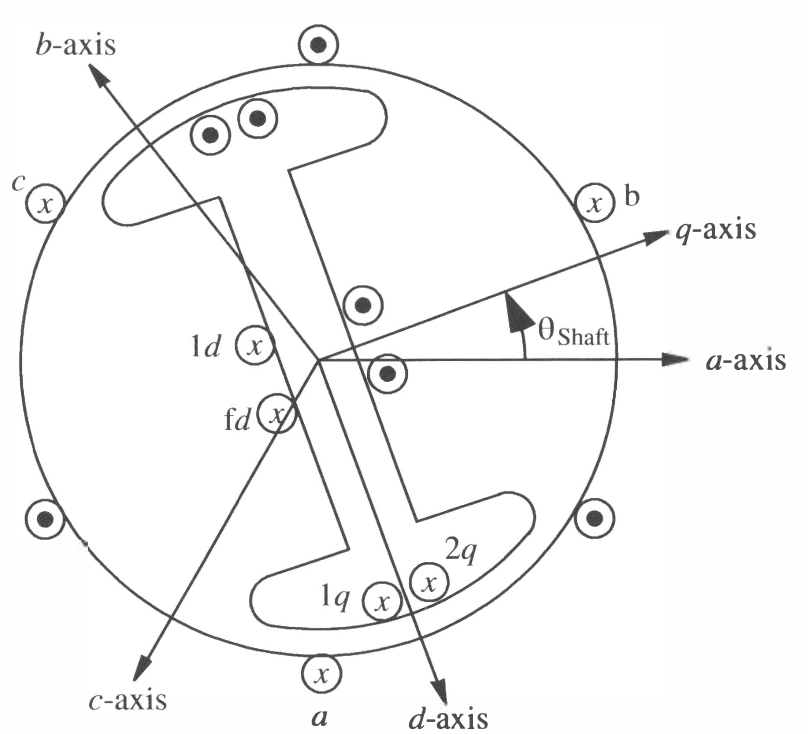
\includegraphics[width = 0.4\textwidth]{images/sg-schematic.png}
    \caption{Schematic diagram of a three-phase synchronous generator \cite{sauer2017power}.}
    \label{fig:sg-schematic}
\end{figure}

\newpage
The assumptions made in the mathematical modeling of the synchronous generators are:
\begin{enumerate}
    \item Stator windings are distributes sinusoidally along the air gap;
    \item Stator slots do not cause any variation in the rotor inductances;
    \item Magnetic hysteresis is negligible;
    \item Magnetic circuit is considered linear.
    \item The rotor has a single pair of poles.
\end{enumerate}

Assumptions 1 to 3 are reasonable since the manufacturing process of synchronous
machines is very precise. Assumption 4 is made for simplification, but in more
complete analysis the nonlinearities of the magnetic circuit should be taken
into account \cite{kundur2022power}. By applying the fundamental Kirchhoff's,
Faraday's and Newton's laws, the following relationships can be derived.

\begin{equation}
    \begin{cases}
        \frac{d\delta}{dt} = \omega_s \Delta\omega\\
        M\frac{\Delta\omega}{dt} = -D\Delta\omega + P_m - P_e\\
        v_a = -i_a r_s + \frac{d\lambda_a}{dt}\\
        v_b = -i_b r_s + \frac{d\lambda_b}{dt}\\
        v_c = -i_c r_s + \frac{d\lambda_c}{dt}\\
        v_{fd} = i_{fd}r_{fd} + \frac{d\lambda_{fd}}{dt}\\
        v_{1d} = i_{1d}r_{1d} + \frac{d\lambda_{1d}}{dt}\\
        v_{1q} = i_{1q}r_{1q} + \frac{d\lambda_{1q}}{dt}\\
        v_{2q} = i_{2q}r_{2q} + \frac{d\lambda_{2q}}{dt}\\
    \end{cases}
    \label{eq:gen_eqs_abc}
\end{equation}

\noindent where $v_{i}$ are the instantaneous phase to neutral voltage, $i_i$
are the currents, $r_{i}$ are the resistances and $\lambda_{i}$ are the flux
linkages in each phase $i$. Moreover, $M$ is the inertia coefficient, $D$ is the
damping coefficient, $P_m$ is the mehchanical torque applied to the shaft, $P_e$
is the electrical torque, $\delta$ is the rotor angle $\theta_{shaft}$ relative
to a rotating frame that rotates with constant speed equal to the synchronous
speed $\omega_s$, and $\Delta\omega = \omega - \omega_s$, where $\omega$ is the
rotor's rotational speed.

\subsection{Linear Magnetic Circuit}

Considering the special case in which the magnetic circuit of the synchronous
generator is linear in relation to the currents, the flux linkages can be
expressed in the following matrix form \cite{siva2022modeling}:

\begin{equation}
    \begin{bmatrix}
        \lambda_a \\ \lambda_b \\ \lambda_c
    \end{bmatrix}
    =
    - \begin{bmatrix}
        l_{aa} & l_{ab} & l_{ac} \\
        l_{ab} & l_{bb} & l_{bc} \\
        l_{ac} & l_{bc} & l_{cc} \\
    \end{bmatrix}
    \begin{bmatrix}
        i_a \\ i_b \\ i_c
    \end{bmatrix}
    + \begin{bmatrix}
        l_{afd} & l_{a1d} & l_{a1q} & l_{a2q}\\
        l_{afd} & l_{b1d} & l_{b1q} & l_{b2q}\\
        l_{afd} & l_{b1d} & l_{c1q} & l_{c2q}\\
    \end{bmatrix}
    \begin{bmatrix}
        i_{fd} \\ i_{1d} \\ i_{1q} \\ i_{2q}
    \end{bmatrix}
    \label{eq:lin_circuit_stator}
\end{equation}

\begin{equation}
    \begin{bmatrix}
        \lambda_{fd} \\ \lambda_{1d} \\ \lambda_{1q} \\ \lambda_{2q}
    \end{bmatrix}
    =
    - \begin{bmatrix}
        l_{fda} & l_{fdb} & l_{fdc} \\
        l_{1da} & l_{1db} & l_{1dc} \\
        l_{1qa} & l_{1qb} & l_{1qc} \\
        l_{2qa} & l_{2qb} & l_{2qc} \\
    \end{bmatrix}
    \begin{bmatrix}
        i_a \\ i_b \\ i_c
    \end{bmatrix}
    + \begin{bmatrix}
        l_{fdfd} & l_{fd1d} & 0 & 0\\
        l_{1dfd} & l_{1d1d} & 0 & 0\\
        0 & 0 & l_{1q1q} & l_{1q2q}\\
        0 & 0 & l_{2q1q} & l_{2q2q}\\
    \end{bmatrix}
    \begin{bmatrix}
        i_{fd} \\ i_{1d} \\ i_{1q} \\ i_{2q}
    \end{bmatrix}
    \label{eq:lin_circuit_rotor}
\end{equation}

Note that the mutual inductances between the $d-$ and $q-$axes are zero, since
they are perpendicular between each other. In normal operation, the angle
between the windings in the rotor and in the stator are constanlty changing,
thus the inductances vary according to the angle $\theta_{shaft}$.

From definition, inductance is equal to the ratio of magnetic flux to current,
magnetic flux is the product of permeance and magnetomotive force, and
magnetomotive force is the product of of the current around the turns and the
number of turns of a coil\cite{purcell2013magnetism}. In other words:

\begin{equation*}
    \begin{aligned}
        l &= \frac{\lambda}{i}\\
        \lambda &= N\phi,\\
        \phi&=FP, \\
        F&=Ni
    \end{aligned}
\end{equation*}

\noindent where $\phi$ is magnetic flux, $N$ is the number of turns of the coil,
$P$ is the permeance and $F$ is the magnetomotive force. In order to understand
how the inductances vary according to $\theta_{shaft}$, let us analyze the
magnetomotive force (mmf) in the $a$-winding of Figure \ref{fig:sg-schematic}.
Let $F_a = N_a i_a$ be the mmf in the $a$-winding, it can be split in the $d-$
and $q-$axes as follows:

\begin{equation}
    \begin{aligned}
        F_{ad} &= F_a \sin{(\theta_{shaft})}\\
        F_{aq} &= F_a \cos{(\theta_{shaft})}
    \end{aligned}
\end{equation}

Let $P_d$ and $P_q$ be the permeances along the $d-$ and $q-$axes, respectively,
the total flux is therefore:

\begin{equation}
    \begin{aligned}
        \phi_{aa} &= F_{ad} P_d \sin{(\theta_{shaft})} + F_{aq} P_q \cos{(\theta_{shaft})}\\
        &= F_{a} P_d \sin^2{(\theta_{shaft})} + F_{a} P_q \cos^2{(\theta_{shaft})}\\
        &= N_a i_a \left(\frac{P_d(1-\cos{(2\theta_{shaft})})}{2} + \frac{P_q(1+\cos{(2\theta_{shaft})})}{2}\right)\\
        &= N_a i_a \left(\frac{P_d + P_q}{2} - \frac{P_d - P_q}{2}\cos{(2\theta_{shaft})}\right) 
    \end{aligned}
\end{equation}

Thus, the self-inductance $l_{aa}$ can be written as:
\begin{equation*}
    l_{aa} = l_{aa0} - l_{aap}\cos{(2\theta_{shaft})}
\end{equation*} 
\noindent where:
\begin{equation*}
    l_{aa0} = N_a^2\left(\frac{P_d + P_q}{2}\right)\;\; \text{and} \;\; l_{aap} = N_a^2\left(\frac{P_d - P_q}{2}\right)
\end{equation*}

Repeating the same procedure for the other windings, the matrices in Equations
\ref{eq:lin_circuit_stator} and \ref{eq:lin_circuit_rotor} become:

\begin{equation*}
    \begin{aligned}
        L_{ss} &= 
        \begin{bmatrix}
            l_{aa} & l_{ab} & l_{ac} \\
            l_{ab} & l_{bb} & l_{bc} \\
            l_{ac} & l_{bc} & l_{cc} \\
        \end{bmatrix}\\
        &=
        \left[\begin{matrix}
        l_{aa0} - l_{aap} \cos{(2\theta_{shaft})} & -\frac{1}{2} l_{aa0} - l_{aap} \cos{(2\theta_{shaft} - \frac{2\pi}{3})} \\
        -\frac{1}{2}l_{aa0} - l_{aap} \cos{(2\theta_{shaft}-\frac{2\pi}{3}}) & l_{aa0} - l_{aap} \cos{(2\theta_{shaft}+\frac{2\pi}{3})}\\
        -\frac{1}{2}l_{aa0} - l_{aap} \cos{(2\theta_{shaft}+\frac{2\pi}{3}}) & -\frac{1}{2} l_{aa0} - l_{aap} \cos{(2\theta_{shaft})}
        \end{matrix}\right.\\
        &\qquad\qquad
        \left.\begin{matrix}
        {}-\frac{1}{2} l_{aa0} - l_{aap} \cos{(2\theta_{shaft} + \frac{2\pi}{3})}\\
        {}-\frac{1}{2} l_{aa0} - l_{aap} \cos{(2\theta_{shaft})}\\
        {}l_{aa0} - l_{aap} \cos{(2\theta_{shaft}-\frac{2\pi}{3})}
        \end{matrix}\right]
    \end{aligned}
\end{equation*}

\begin{equation*}
    \begin{aligned}
        L_{sr} &= 
        \begin{bmatrix}
            l_{afd} & l_{a1d} & l_{a1q} & l_{a2q}\\
            l_{afd} & l_{b1d} & l_{b1q} & l_{b2q}\\
            l_{afd} & l_{b1d} & l_{c1q} & l_{c2q}\\
        \end{bmatrix}\\
        &=
        \left[\begin{matrix}
        l_{sfd}\sin(\theta_{shaft}) & l_{s1d}\sin(\theta_{shaft})\\
        l_{sfd}\sin(\theta_{shaft}-\frac{2\pi}{3}) & l_{s1d}\sin(\theta_{shaft}-\frac{2\pi}{3})\\
        l_{sfd}\sin(\theta_{shaft}+\frac{2\pi}{3}) & l_{s1d}\sin(\theta_{shaft}+\frac{2\pi}{3})\\
        \end{matrix}\right.\\
        &\qquad\qquad
        \left.\begin{matrix}
        {}l_{s1q}\cos(\theta_{shaft}) & l_{s2q}\cos(\theta_{shaft})\\
        {}l_{s1q}\cos(\theta_{shaft}-\frac{2\pi}{3}) & l_{s2q}\cos(\theta_{shaft}-\frac{2\pi}{3})\\
        {}l_{s1q}\cos(\theta_{shaft}+\frac{2\pi}{3}) & l_{s2q}\cos(\theta_{shaft}+\frac{2\pi}{3})
        \end{matrix}\right]
    \end{aligned}
\end{equation*}

\noindent where:
\begin{equation*}
    \begin{aligned}
        l_{afd} = l_{bfd} = l_{cfd} = l_{sfd}\\
        l_{a1d} = l_{b1d} = l_{c1d} = l_{s1d}\\
        l_{a1q} = l_{b1q} = l_{c1q} = l_{s1q}\\
        l_{a2q} = l_{b2q} = l_{c2q} = l_{s2q}\\
    \end{aligned}
\end{equation*}

Since the above matrices vary with $\theta_{shaft}$, it is convenient to make a
coordinate transformation to a rotating reference system with same speed as
$\theta_{shaft}$ so that the trigonometrical terms disappear. This coordinate
transformation is referred to Park's transformation (or $dq0-$transformation)
and drastically reduces the complexity of the equations.

\subsection{Park's Transformation (\textit{dq0}-transformation)}

In power systems, the $dq0$-transformation, also known as Park's transformation,
consists in converting from the static \textit{abc} frame to a rotating $dq0$
frame. The main objective of this transformation is to reduce a three-phase
sinusoidal components into two-dimensional DC components, and therefore it
results in relatively simple dynamic models that can be controlled through
classical PID controllers.

This transformation slightly differs from author to author depending on the
choice of the leading and lagging components. For instance, in
\cite{sauer2017power} the authors consider the a-axis and the q-axis initially
aligned, while in \cite{krause2002analysis} the authors considers the a-axis and
the d-axis initially aligned.

\begin{figure}[!ht]
    \centering
    \begin{subfigure}{.5\textwidth}
      \centering
      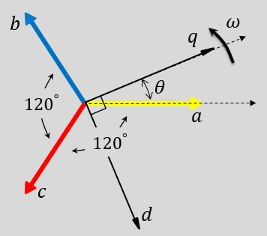
\includegraphics[width=5cm]{images/park_transform_axes_01.png}
      \caption{The a-axis and the q-axis are initially aligned.}
      \label{fig:park_transform_axes_01}
    \end{subfigure}%
    \begin{subfigure}{.5\textwidth}
      \centering
      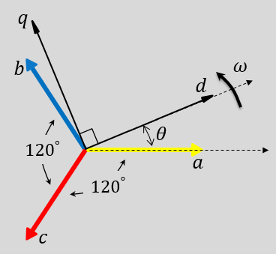
\includegraphics[width=5cm]{images/park_transform_axes_02.png}
      \caption{The a-axis and the d-axis are initially aligned.}
      \label{fig:park_transform_axes_2}
    \end{subfigure}
    \caption{Different representations of \textit{dq0} frame.}
    \label{fig:park_transform_axes}
\end{figure}

In this thesis, the a-axis and the q-axis are chosen to be initially aligned. In this
case, the Park transformation can be expressed by the following transformation matrix
from $abc$ frame to the rotating $dq0$ frame.

\begin{equation}
    T_{dq0} = 
    \frac{2}{3}
    \begin{bmatrix}
        \sin{(\theta)} & \sin{\left(\theta - \frac{2\pi}{3}\right)} & \sin{\left(\theta + \frac{2\pi}{3}\right)}\\
        \cos{(\theta)} & \cos{\left(\theta - \frac{2\pi}{3}\right)} & \cos{\left(\theta + \frac{2\pi}{3}\right)}\\
        \frac{1}{2} & \frac{1}{2} & \frac{1}{2}
    \end{bmatrix}
    \label{eq:park_transformation}
\end{equation}

The inverse transformation can be expressed by the following matrix.

\begin{equation}
    T_{dq0}^{-1} = 
    \begin{bmatrix}
        \sin{(\theta)} & \cos{(\theta)} & 1 \\
        \sin{(\theta-\frac{2\pi}{3})} & \cos{(\theta-\frac{2\pi}{3})} & 1 \\
        \sin{(\theta+\frac{2\pi}{3})} & \cos{(\theta+\frac{2\pi}{3})} & 1 \\
    \end{bmatrix}
    \label{eq:park_inverse_transformation}
\end{equation}

Applying this transformation to the stator voltages, i.e. the first three
equations in Equation \ref{eq:gen_eqs_abc}:

\begin{equation*}
    \begin{aligned}
        \begin{bmatrix}
            v_d \\ v_q \\ v_0
        \end{bmatrix}
        &= -T_{dq0}
        \begin{bmatrix}
            r_s & 0 & 0\\
            0 & r_s & 0\\
            0 & 0 & r_s
        \end{bmatrix}
        T_{dq0}^{-1}
        \begin{bmatrix}
            i_d \\ i_q \\ i_0
        \end{bmatrix}
        +
        T_{dq0}\frac{d}{dt}\left(T_{dq0}^{-1}\begin{bmatrix}\lambda_d \\ \lambda_q\\ \lambda_0\end{bmatrix}\right)\\
        &= -
        \begin{bmatrix}
            r_s & 0 & 0\\
            0 & r_s & 0\\
            0 & 0 & r_s
        \end{bmatrix}
        \begin{bmatrix}
            i_d \\ i_q \\ i_0
        \end{bmatrix}
        +
        T_{dq0}\frac{dT_{dq0}^{-1}}{dt}\left(\begin{bmatrix}\lambda_d \\ \lambda_q\\ \lambda_0\end{bmatrix}\right) + \frac{d}{dt} \left(\begin{bmatrix}\lambda_d \\ \lambda_q\\ \lambda_0\end{bmatrix}\right) \\ 
        &= -
        \begin{bmatrix}
            r_s & 0 & 0\\
            0 & r_s & 0\\
            0 & 0 & r_s
        \end{bmatrix}
        \begin{bmatrix}
            i_d \\ i_q \\ i_0
        \end{bmatrix}
        +
        \begin{bmatrix}
            0 & -\omega & 0 \\
            \omega & 0 & 0 \\
            0 & 0 & 0
        \end{bmatrix}\begin{bmatrix}\lambda_d \\ \lambda_q\\ \lambda_0\end{bmatrix}
        +
        \frac{d}{dt} \left(\begin{bmatrix}\lambda_d \\ \lambda_q\\ \lambda_0\end{bmatrix}\right) \\ 
    \end{aligned}
\end{equation*}

Therefore, the Equation \ref{eq:gen_eqs_abc} in the $dq0$ coordinates has the forms:
\begin{equation}
    \begin{cases}
        \frac{d\delta}{dt} = \omega_s \Delta\omega\\
        M\frac{\Delta\omega}{dt} = -D\Delta\omega + P_m - P_e\\
        v_d = -r_s i_d - \omega\lambda_q + \frac{d\lambda_d}{dt}\\
        v_q = -r_s i_q + \omega\lambda_d + \frac{d\lambda_q}{dt}\\
        v_0 = -r_s i_0 + \frac{d\lambda_0}{dt}\\
        v_{fd} = r_{fd} i_{fd} + \frac{d\lambda_{fd}}{dt}\\
        v_{1d} = r_{1d} i_{1d} + \frac{d\lambda_{1d}}{dt}\\
        v_{1q} = r_{1q} i_{1q} + \frac{d\lambda_{1q}}{dt}\\
        v_{2q} = r_{2q} i_{2q} + \frac{d\lambda_{2q}}{dt}\\
    \end{cases}
    \label{eq:gen_eqs_dq0}
\end{equation}

% TODO: improve this passage
Moreover, in order to calculate the stator fluxes in the $dq0$ coordinates, let
us apply the transformations \ref{eq:park_transformation} and
\ref{eq:park_inverse_transformation} to Equations \ref{eq:lin_circuit_stator}
and \ref{eq:lin_circuit_rotor}. For the explicit calculation, please refer to
\cite{krause2002analysis}.

\begin{equation}\label{eq:fluxes_dq0}
    \begin{aligned}
        \lambda_d &= -(l_{md} + l_{ls}) i_d + l_{sfd} i_{fd} + l_{s1d}i_{1d}\\
        \lambda_q &= -(l_{mq} + l_{ls}) i_d + l_{s1q} i_{fd} + l_{s2q}i_{1d}\\
        \lambda_{0} &= -l_{ls} i_0\\
        \lambda_{fd} &= -\frac{3}{2} l_{sfd}i_d + l_{fdfd}i_{fd} + l_{fd1d}i_{1d}\\
        \lambda_{1d} &= -\frac{3}{2} l_{s1d}i_d + l_{fd1d}i_{fd} + l_{1d1d}i_{1d}\\
        \lambda_{1q} &= -\frac{3}{2} l_{s1q}i_q + l_{1q1q}i_{1q} + l_{1q2q}i_{2q}\\
        \lambda_{2q} &= -\frac{3}{2} l_{s2q}i_q + l_{1q2q}i_{1q} + l_{2q2q}i_{2q}\\
    \end{aligned}
\end{equation}

\noindent where $l_{md}$, $l_{mq}$ and $l_{ls}$ are, respectively, the mutual
inductance in the $d-$ and $q-$axes and the leakage inductance.

\subsection{Per-Unit System}

In power system studies, it is customary to scale all quantities using the
per-unit system. Typically, voltage and power are selected based on the
equipment ratings, and base values such as current and impedance are derived
from these. When studying a system, a convenient round number, such as 100 MVA,
is often chosen as the base power, and the base voltage is usually set to the
nominal rated value of the system. The key advantages of employing a per-unit
system include:

\begin{itemize}
    \item \textbf{Ease of comparison:} the per-unit system eliminates differences
    in power and voltage drops across a circuit, allowing for the comparison of
    losses and performance among different equipment based on their impedances
    in per units.
    \item \textbf{Simplification of circuits with transformers:} in power
    systems with transformers, converting a transformer into its equivalent
    circuit on either the primary or secondary side is necessary. However, using
    per-unit systems makes the impedances referred to either side of a
    transformer identical, eliminating the need to calculate impedances on both
    sides.
    \item \textbf{Elimination of multiple voltage levels:} in power systems with
    multiple transformers, the per-unit system reduces all voltage levels to a
    single level, simplifying calculations by referencing all impedances to this
    level.
    \item \textbf{Elimination of $\sqrt{3}$ in three-phase circuits:} Per-unit
    systems eliminate the need for the $\sqrt{3}$ factor in three-phase systems,
    avoiding errors and simplifying calculations that involve per-phase and
    line-to-line conversions.
\end{itemize}

Due to the composition of multiple coils in its stator and rotor, a synchronous
generator can be treated as multiple transformers, each with different voltage
levels. Therefore, the use of a per-unit system is highly beneficial for
analyzing synchronous generators, ensuring that rotor and stator quantities are
referred to the same base. 

In the subsequent subsections, Equations \ref{eq:gen_eqs_dq0} and
\ref{eq:fluxes_dq0} are reformulated in the per-unit system, giving rise to the
Park's model of a synchronous generator, also known as the detailed model.
Subject to certain assumptions, this detailed model will be further reduced into
the 2-axis, 1-axis, and classical models of a synchronous generator. For a
detailed explanation of the reformulation of Equations \ref{eq:gen_eqs_dq0} and
\ref{eq:fluxes_dq0} in the per-unit system, please refer to
\cite{sauer2017power} and \cite{siva2022modeling}.

% TODO: how to explain the variables of these equations?
\subsection{Park's Model (Detailed Model)}

The Park's model, also known as the detailed model, corresponds to Equations
\ref{eq:gen_eqs_dq0} and \ref{eq:fluxes_dq0} reformulated in the per-unit
system. It represents a 9th-order system comprising 2 mechanical equations
describing rotor motion and 7 electromechanical equations describing the three
stator windings and four rotor windings (one field winding, and one damper
winding on the $d$-axis, and two damper windings on the $q$-axis).

\begin{equation}\label{eq:sg_park}
    \begin{cases}
        \frac{d\delta}{dt} &= \omega_s \Delta\omega\\
        M\frac{\Delta\omega}{dt} &= -D\Delta\omega + P_m - P_e\\
        \frac{1}{\omega_s} \frac{d\psi_d}{dt} &= R_s I_d + \frac{\omega}{\omega_s}\psi_q + V_d\\
        \frac{1}{\omega_s} \frac{d\psi_q}{dt} &= R_s I_q - \frac{\omega}{\omega_s}\psi_d + V_q\\
        \frac{1}{\omega_s} \frac{d\psi_0}{dt} &= R_s I_0 + V_0\\
        T_{do}'\frac{dE_q}{dt} &= -E_q - (X_d - X_d')\left(I_d - \frac{(X_d' - X_d'')}{(X_d' - X_{ls})^2}(\psi_{1d} +\right.\\
                               &+ \left. (X_d' - X_{ls})I_d - E_q\right) + E_{fd}\\
        T_{do}''\frac{d\psi_{1d}}{dt} &= -\psi_{1d} + E_q - (X_d' - X_{ls}) I_d\\
        T_{qo}'\frac{dE_d}{dt} &= -E_d - (X_q - X_q')\left(I_q - \frac{(X_q' - X_q'')}{(X_q' - X_{ls})^2}(\psi_{2q} +\right.\\
                               &+ \left. (X_q' - X_{ls})I_q + E_d\right)\\
        T_{qo}''\frac{d\psi_{2q}}{dt} &= -\psi_{2q} - E_d - (X_q' - X_{ls}) I_q\\
        \psi_d &= -X_d'' I_d + \frac{(X_d'' - X_{ls})}{(X_d' - X_{ls})} E_q + \frac{(X_d' - X_d'')}{(X_d' - X_{ls})}\psi_{1d}\\
        \psi_q &= -X_q'' I_q - \frac{(X_q'' - X_{ls})}{(X_q' - X_{ls})} E_d + \frac{(X_q' - X_q'')}{(X_q' - X_{ls})}\psi_{2q}\\
        \psi_0 &= -X_{ls} I_0\\
    \end{cases}
\end{equation}

% \noindent where the 
% \begin{align*}
%     \delta & : \text{Rotor angle (measured in radians)} \\
%     \Delta\omega & : \text{Deviation in rotor speed (angular frequency)} \\
%     M & : \text{Inertia constant} \\
%     D & : \text{Damping factor} \\
%     P_m & : \text{Mechanical power input} \\
%     P_e & : \text{Electrical power output} \\
%     \psi_d & : \text{Direct-axis stator flux} \\
%     \psi_q & : \text{Quadrature-axis stator flux} \\
%     \psi_0 & : \text{Zero-sequence stator flux} \\
%     \psi_{1d} & : \text{First damper winding flux on the } d\text{-axis} \\
%     \psi_{2q} & : \text{Second and third damper winding fluxes on the } q\text{-axis} \\
%     I_d & : \text{Direct-axis stator current} \\
%     I_q & : \text{Quadrature-axis stator current} \\
%     I_0 & : \text{Zero-sequence stator current} \\
%     V_d & : \text{Direct-axis stator voltage} \\
%     V_q & : \text{Quadrature-axis stator voltage} \\
%     V_0 & : \text{Zero-sequence stator voltage} \\
%     \omega_s & : \text{Synchronous angular frequency} \\
%     R_s & : \text{Stator resistance} \\
%     X_d & : \text{Direct-axis synchronous reactance} \\
%     X_d' & : \text{Direct-axis transient reactance} \\
%     X_d'' & : \text{Direct-axis subtransient reactance} \\
%     X_{ls} & : \text{Leakage reactance} \\
%     T_{do}' & : \text{Direct-axis open-circuit time constant} \\
%     T_{do}'' & : \text{Direct-axis short-circuit time constant} \\
%     T_{qo}' & : \text{Quadrature-axis open-circuit time constant} \\
%     T_{qo}'' & : \text{Quadrature-axis short-circuit time constant} \\
%     E_q & : \text{Quadrature-axis stator voltage (induced)} \\
%     E_{fd} & : \text{Field voltage} \\
%     E_d & : \text{Direct-axis stator voltage (induced)} \\
%     E_d' & : \text{Transient direct-axis stator voltage} \\
% \end{align*}

\subsection{2-axis Model (Subtransient Model)}

The Park's model can be reduced to a 4th-order system, also known as the 2-axis
model (or subtransient model), by eliminating the stator/network transients and 
assuming that the short-circuit time constants $T_{do}''$ and $T_{qo}''$ are
sufficiently small \cite{sauer2017power}.

First, the stator/network transients can be eliminated by assuming that
$\omega_s$ is large enough such that $\frac{1}{\omega_s} \approx 0$. Then, the
stator/network fluxes in Equation \ref{eq:sg_park} become.

\begin{equation*}
    \begin{cases}
        0 &= R_s I_d + \frac{\omega}{\omega_s}\psi_q + V_d\\
        0 &= R_s I_q - \frac{\omega}{\omega_s}\psi_d + V_q\\
        0 &= R_s I_0 + V_0\\
        \psi_d &= -X_d'' I_d + \frac{(X_d'' - X_{ls})}{(X_d' - X_{ls})} E_q + \frac{(X_d' - X_d'')}{(X_d' - X_{ls})}\psi_{1d}\\
        \psi_q &= -X_q'' I_q - \frac{(X_q'' - X_{ls})}{(X_q' - X_{ls})} E_d + \frac{(X_q' - X_q'')}{(X_q' - X_{ls})}\psi_{2q}\\
        \psi_0 &= -X_{ls} I_0\\
    \end{cases}
\end{equation*}

The solution of the above equations of $\psi_0$ and $I_0$ is trivial, and
$\psi_d$ and $\psi_q$ can be eliminated, leaving only the following two
equations to be solved for $I_d$ and $I_q$.

\begin{equation}\label{eq:for_I_2axis}
    \begin{cases}
        0 &= R_s I_d - X_q'' I_q - \frac{(X_q'' - X_{ls})}{(X_q' - X_{ls})} E_d + \frac{(X_q' - X_q'')}{(X_q' - X_{ls})}\psi_{2q} + V_d \\
        0 &= R_s I_q - X_d'' I_d - \frac{(X_d'' - X_{ls})}{(X_d' - X_{ls})} E_q - \frac{(X_d' - X_d'')}{(X_d' - X_{ls})}\psi_{1d} + V_q \\
    \end{cases}
\end{equation}

Moreover, assuming that the short-circuit time constants $T_{do}''$ and
$T_{qo}''$ are sufficiently small, the damping winding dynamic equations in
Equation \ref{eq:sg_park} become:

\begin{equation*}
    \begin{cases}
        0 &= -\psi_{1d} + E_q - (X_d' - X_{ls}) I_d\\
        0 &= -\psi_{2q} - E_d - (X_q' - X_{ls}) I_q\\
    \end{cases}
\end{equation*}

Replacing $\psi_{1d}$ and $\psi_{2q}$ in Equation \ref{eq:for_I_2axis}:
\begin{equation*}
    \begin{cases}
        0 &= R_s I_d - X_q' I_q - E_d + V_d \\
        0 &= R_s I_q + X_d' I_d - E_q + V_q \\
    \end{cases}
\end{equation*}

Finally, the Park's model is reduced to the two-axis model, also known as
substransient model, and it is expressed by the following set of dynamical
equations.

\begin{equation} \label{eq:sg_two_axis}
    \begin{cases}
        \frac{d\delta}{dt} &= \omega_s \Delta\omega\\
        M\frac{\Delta\omega}{dt} &= -D\Delta\omega + P_m - P_e\\
        T_{do}' \frac{E_q}{dt} &= -E_q - (X_d - X_d')I_d + E_{fd}\\
        T_{qo}' \frac{E_d}{dt} &= -E_d + (X_q - X_q')I_q\\
        0 &= R_s I_d - X_q' I_q - E_d + V_d \\
        0 &= R_s I_q + X_d' I_d - E_q + V_q
    \end{cases}
\end{equation}

\subsection{1-axis Model (Flux-Decay Model)}

The 2-axis model still considers the dynamics of the damper winding $1q$
illustrated in Figure \ref{fig:sg-schematic}. Similarly to the approximation
made for eliminating the damper windings $1d$ and $2q$ in the previous
subsection, if $T_{qo}'$ is sufficiently small, the dynamic equation of the
damper winding $1q$ becomes:

\begin{equation*}
    0 = -E_d + (X_q - X_q')I_q
\end{equation*}

Replacing $E_d$ in the algebraic equations for $I_d$ and $I_q$, the model
described by Equation \ref{eq:sg_two_axis} becomes:

\begin{equation} \label{eq:sg_one_axis}
    \begin{cases}
        \frac{d\delta}{dt} &= \omega_s \Delta\omega\\
        M\frac{\Delta\omega}{dt} &= -D\Delta\omega + P_m - P_e\\
        T_{do}' \frac{E_q}{dt} &= -E_q - (X_d - X_d')I_d + E_{fd}\\
        0 &= R_s I_d - X_q I_q + V_d \\
        0 &= R_s I_q + X_d' I_d - E_q + V_q
    \end{cases}
\end{equation}

\noindent which is often called the 1-axis (or flux-decay) synchronous machine
model.

% TODO: verify if the derivation of classical model is correct
\subsection{Classical Model}

Finally, the classical model is a further simplification considering $T_{do}'$
sufficiently small, and therefore the dynamic equation of the excitation winding
can be ignored in the similar way as in the previous two subsections. In other
words, the classical model only considers the mechanical dynamics of the
synchronous generator, and can be described by the following set of equations.

\begin{equation} \label{eq:sg_classical}
    \begin{cases}
        \frac{d\delta}{dt} &= \omega_s \Delta\omega\\
        M\frac{\Delta\omega}{dt} &= -D\Delta\omega + P_m - P_e\\
        0 &= R_s I_d - X_q I_q + V_d \\
        0 &= R_s I_q + X_d I_d + V_q
    \end{cases}
\end{equation}

\section{Modeling of Exciter and Automatic Voltage Regulator (AVR)}
\section{Modeling of Turbine/Governor}

\section{Power System Stabilizer (PSS)}
\section{Automatic Generation Control (AGC)}